\documentclass{article}

\setlength{\headsep}{0.75 in}
\setlength{\parindent}{0 in}
\setlength{\parskip}{0.1 in}

%=====================================================
% Add PACKAGES Here (You typically would not need to):
%=====================================================

\usepackage{xcolor}
\usepackage[margin=1in]{geometry}
\usepackage{amsmath,amsthm}
\usepackage{fancyhdr}
\usepackage{enumitem}
\usepackage{graphicx}

%=====================================================
% Ignore This Part (But Do NOT Delete It:)
%=====================================================

\theoremstyle{definition}
\newtheorem{problem}{Problem}
\newtheorem*{fun}{Fun with Algorithms}
\newtheorem*{challenge}{Challenge Yourself}
\def\fline{\rule{0.75\linewidth}{0.5pt}}
\newcommand{\finishline}{\begin{center}\fline\end{center}}
\newtheorem*{solution*}{Solution}
\newenvironment{solution}{\begin{solution*}}{{\finishline} \end{solution*}}
\newcommand{\grade}[1]{\hfill{\textbf{($\mathbf{#1}$ points)}}}
\newcommand{\thisdate}{\today}
\newcommand{\thissemester}{\textbf{Rutgers: Spring 2021}}
\newcommand{\thiscourse}{CS 344: Design and Analysis of Computer Algorithms} 
\newcommand{\thishomework}{Number} 
\newcommand{\thisname}{Name} 
\newcommand{\thisextension}{Yes/No} 

\headheight 40pt              
\headsep 10pt
\renewcommand{\headrulewidth}{0pt}
\lhead{\small \textbf{Only for the personal use of students registered in CS 344, Spring 2021 at Rutgers University. Redistribution out of this class is strictly prohibited.}}
\pagestyle{fancy}

\newcommand{\thisheading}{
   \noindent
   \begin{center}
   \framebox{
      \vbox{\vspace{2mm}
    \hbox to 6.28in { \textbf{\thiscourse \hfill \thissemester} }
       \vspace{4mm}
       \hbox to 6.28in { {\Large \hfill Homework \#\thishomework \hfill} }
       \vspace{2mm}
         \hbox to 6.28in { { \hfill \thisdate  \hfill} }
       \vspace{2mm}
       \hbox to 6.28in { \emph{Name: \thisname \hfill Extension: \thisextension}}
      \vspace{2mm}}
      }
   \end{center}
   \bigskip
}

%=====================================================
% Some useful MACROS (you can define your own in the same exact way also)
%=====================================================


\newcommand{\ceil}[1]{{\left\lceil{#1}\right\rceil}}
\newcommand{\floor}[1]{{\left\lfloor{#1}\right\rfloor}}
\newcommand{\prob}[1]{\Pr\paren{#1}}
\newcommand{\expect}[1]{\Exp\bracket{#1}}
\newcommand{\var}[1]{\textnormal{Var}\bracket{#1}}
\newcommand{\set}[1]{\ensuremath{\left\{ #1 \right\}}}
\newcommand{\poly}{\mbox{\rm poly}}


%=====================================================
% Fill Out This Part With Your Own Information:
%=====================================================


\renewcommand{\thishomework}{1} %Homework number
\renewcommand{\thisname}{Letao Zhang} % Enter your name here
\renewcommand{\thisextension}{No} % Pick only one of the two options accordingly

\begin{document}

\thisheading
\vspace{-0.75cm}


%=====================================================
% LaTeX Tip: You can erase this part from here.... 
%=====================================================		

\subsection*{Homework Policy}
\begin{itemize}
\item If you leave a question completely blank, you will receive 25\% of the grade for that question. This however does not apply to the extra credit questions.
\item You are allowed to discuss the homework problems with other students in the class. \textbf{But you must write your solutions independently.} 
You may also consult all the materials used in this course (video recordings, notes, textbook, etc.) while writing your solution, but no other resources are allowed.
\item Do not forget to write down your name and whether or not you are using one of your two extensions. Submit your homework on Canvas. 
\item Unless  specified otherwise, you may use any algorithm covered in class as a ``black box'' -- for example you can simply write ``sort the array in $\Theta(n\log{n})$ time using merge sort''.
\item Remember to always \textbf{prove the correctness} of your algorithms and \textbf{analyze their running time} (or any other efficiency measure asked in the question). See ``Practice Homework'' for an example.  

\item The ``Challenge yourself'' and ``Fun with algorithms''  are both extra credit. These problems are significantly more challenging than the standard problems you see in this course (including lectures, homeworks, and exams). 
As a general rule, only attempt to solve these problems if you  enjoy them. 
\end{itemize}

\finishline

%=====================================================
% LaTeX Tip: ... to here
%=====================================================	


\bigskip

\begin{problem}
	This question reviews asymptotic notation. You may assume the following inequalities for this question (and throughout the course): For any \underline{constant} $c \geq 1$, 
	\begin{align*}
		(\log{n})^c = o(n) \quad,\quad n^c = o(n^{c+1}) \quad,\quad c^n = o((c+1)^n) \quad,\quad (n/2)^{(n/2)} = o(n!) \quad,\quad n! = o(n^n). 
	\end{align*}
	\begin{enumerate}
	\item[(a)] Rank the following functions based on their asymptotic value in the increasing order, i.e., list them as functions $f_1,f_2,f_3,\ldots,f_{9}$ such that $f_1 = O(f_2)$, $f_2 = O(f_3), \ldots, f_{8} = O(f_{9})$. Remember to write down your proof
	for each equation $f_i = O(f_{i+1})$ in the sequence above.  \grade{15}
	\begin{align*}
		&\sqrt{\log{n}} &&\log\log{n} &&2^{{\log{n}}}  \\ 
		&100n   &&10^{n} &&2^{2^{2^{2^{2}}}} \\ 
		&2^{n} && n! &&\frac{n}{\log{n}} 
	\end{align*}
	
	\smallskip 
	\emph{Hint:} For some of the proofs, you can simply show that $f_i(n) \leq f_{i+1}(n)$ for all \underline{sufficiently large} $n$ which immediately implies $f_i = O(f_{i+1})$. 
	
%=====================================================
% LaTeX Tip: Write your solutions for each problem in a solution environment, i.e., between a \begin{solution} and \end{solution} command. For problems that have multiple part, use this command right after each part
% of the problem.  
%=====================================================	

\begin{solution}

	\begin{align*} 
		&f_1 = \sqrt{\log{n}} &&f_2 = \log\log{n} = O(\log\log{n}) &&f_3 = 2^{{\log{n}}} < O(n)  \\ 
		&f_4 = 100n =O(n) &&f_5 = 10^{n} = O(10^{n}) &&f_6 = 2^{2^{2^{2^{2}}}} = O(1) \\ 
		&f_7 = 2^{n} = O(2^{n}) &&f_8 = n! = O(n^{n}) &&f_9 = \frac{n}{\log{n}} 
	\end{align*}
	Rank: $f_6 < f_2 < f_1 < f_3 < f_9 < f_4 < f_7 < f_5 < f_8$ \\
	
\end{solution}
	
	\item[(b)]  Consider the following four different functions $f(n)$: 
	  \begin{align*}
	    1 \qquad\qquad  \log n \qquad\qquad  n^2  \qquad\qquad  4^{4^{n}}.
	  \end{align*} 
	 For each of these functions, determine which of the following statements is true and which one is false. Remember to write down your proof for each choice.    \grade{10} 
	\begin{itemize}
        \item $f(n) = \Theta(f(n-1))$;
        \item $f(n) = \Theta(f(\frac{n}{2}))$;
        \item $f(n) = \Theta(f(\sqrt n))$;
    \end{itemize}
    
    \smallskip
	\textbf{Example:} For the function $f(n) = 4^{4^n}$, we have $f(n-1) = 4^{4^{n-1}}$.  Since $4^{4^{n-1}}= 4^{\frac{1}{4} \cdot 4^n} = (4^{4^{n}})^{1/4}$.
	\[
		\lim_{n \to \infty}\frac{f(n)}{f(n-1)} = \lim_{n \to \infty}\frac{4^{4^{n}}}{4^{4^{n-1}}} = \lim_{n \to \infty}\frac{4^{4^{n}}}{(4^{4^{n}})^{1/4}} = \lim_{n \to \infty}(4^{4^{n}})^{3/4} = +\infty.
	\]	
	As such, $f(n) \neq O(f(n-1))$ and thus the first statement is false for $4^{4^n}$.

    \end{enumerate}
    
    \begin{solution} .\\
    
  	 1) For the function $f(n) = 1$; we know that 
	 \[ 
	 	\lim_{n \to \infty}\frac{1}{1} = 1.
	\] 
	 As such, all cases are true. \\

	 2) For the function $f(n) = \log n$. \\
	 
	 	a) We know that $f(n-1) = \log(n -1)$. 
	 	\[
			\lim_{n \to \infty}\frac{f(n)}{f(n-1)} = \lim_{n \to \infty}\frac{\log n}{\log(n -1)} = \lim_{n \to \infty}\frac{\frac{1}{n}}{\frac{1}{n-1}} = \lim_{n \to \infty}1 - \frac{1}{n} = 1.
		\]	
			As such, $f(n) = O(f(n-1))$ and thus the first statement is true. \\ 
			
	 	b) We know that $f(\frac{n}{2}) = \log(\frac{n}{2})$. 
	 	\[
			\lim_{n \to \infty}\frac{f(n)}{f(\frac{n}{2})} = \lim_{n \to \infty}\frac{\log n}{\log n - \log 2} = \lim_{n \to \infty}\frac{\log n}{\log n - \log 2} = 1.
		\]	
			As such, $f(n) = O(f(\frac{n}{2}))$ and thus the second statement is true. \\ 
		
		c) We know that $f(\sqrt n) = \log(\sqrt n) = \frac{1}{2} \log n$. 
	 	\[
			\lim_{n \to \infty}\frac{f(n)}{f(\sqrt n)} = \lim_{n \to \infty}\frac{\log n}{\frac{1}{2} \log n} = \lim_{n \to \infty}2 = 2.
		\]	
			As such, $f(n) = O(f(\sqrt n)$ and thus the third statement is true. \\ 
		
		
	 3) For the function $f(n) =  n^2$. \\
	 
	 a) We know that $f(n-1) = (n -1)^2 = n^2 + 2n -1$. 
	 \[
		\lim_{n \to \infty}\frac{f(n)}{f(n-1)} = \lim_{n \to \infty}\frac{n^2}{n^2 + 2n -1} = \lim_{n \to \infty}\frac{2n}{2n - 2} = \lim_{n \to \infty}\frac{2}{2} = 1.
	\]	
		As such, $f(n) = O(f(n-1))$ and thus the first statement is true. \\
		
	b) We know that $f(\frac{n}{2}) = (\frac{n}{2})^2 = \frac{n^2}{4} $. 
	 	\[
			\lim_{n \to \infty}\frac{f(n)}{f(\frac{n}{2})} = \lim_{n \to \infty}\frac{n^2}{\frac{n^2}{4}} = 4.
		\]	
			As such, $f(n) = O(f(\frac{n}{2}))$ and thus the second statement is true. \\ 
		
	c) We know that $f(\sqrt n) = \sqrt(n^2) = n$. 
	 	\[
			\lim_{n \to \infty}\frac{f(n)}{f(\sqrt n)} = \lim_{n \to \infty}\frac{n^2}{n} = \lim_{n \to \infty}n = \infty.
		\]	
			As such, $f(n) = O(f(\sqrt n)$ and thus the third statement is false. \\ 
	 
	 4) For the function $f(n) = 4^{4^n}$. \\ 
	  
	 a) We know that  $f(n-1) = 4^{4^{n-1}}$.  Since $4^{4^{n-1}}= 4^{\frac{1}{4} \cdot 4^n} = (4^{4^{n}})^{1/4}$.
	\[
		\lim_{n \to \infty}\frac{f(n)}{f(n-1)} = \lim_{n \to \infty}\frac{4^{4^{n}}}{4^{4^{n-1}}} = \lim_{n \to \infty}\frac{4^{4^{n}}}{(4^{4^{n}})^{1/4}} = \lim_{n \to \infty}(4^{4^{n}})^{3/4} = +\infty.
	\]	
		As such, $f(n) \neq O(f(n-1))$ and thus the first statement is false. \\
		
	b) We know that $f(\frac{n}{2}) = 4^{4^{\frac{n}{2}}}$.
	 \[
		\lim_{n \to \infty}\frac{f(n)}{f(\frac{n}{2})} = \lim_{n \to \infty}\frac{4^{4^n}}{4^{4^{\frac{n}{2}}}} = \infty.
	\]	
		As such, $f(n) \neq O(f(\frac{n}{2}))$ and thus the second statement is false. \\ 
		
	c) We know that $f(\sqrt n) = 4^{4^{\sqrt n}}$.
	 \[
		\lim_{n \to \infty}\frac{f(n)}{f(\sqrt n)} = \lim_{n \to \infty}\frac{4^{4^n}}{4^{4^{\sqrt n}}} = \infty.
	\]	
		As such, $f(n) \neq O(f(\sqrt n)$ and thus the third statement is false. \\ 
	 
\end{solution}

%=====================================================
% LaTeX Tip: Feel free to erase the Example/Hint parts when writing your solution if they are in the way (when doing so, make sure you do not erase the
% other parts of LaTeX commands such as \end{enumerate} or \end{problem} -- however, please NEVER erase the problem statements. 
%=====================================================		


\end{problem}


\smallskip


		
\begin{problem}
	Your goal in this problem is to analyze the \emph{runtime} of the following (imaginary) recursive algorithms for some (even more imaginary) problem:
	\begin{enumerate}[label=(\Alph*)]
	
		\item Algorithm $A$ divides an instance of size $n$ into $4$ subproblems of size $n/4$ each, recursively solves each one, and then takes $O(n)$ time 
		to combine the solutions and output the answer.
		
		    \begin{solution}
			
			\emph{Runtime Analysis}
	
	%=====================================================
% LaTeX Tip: The figure environment is used for displaying the figure. Inside that, we use \includegraphics for adding a different file for each of the figure.
% What you need to do is to create your figure using any tool you like (including drawing it by hand and scanning it), turn it into a pdf, name it "tree[X].pdf" 
% where you replace [X] by A,B,C, or D depending on which part you are solving (i.e., use treeA.pdf, treeB.pdf,...). Finally, copy the file in the same directory
% as this template and you should see that getting compiled into your solution. You can change the width=0.5\textwidth command to fix the size of the figure
% in the final PDF. Finally, if the figure appears in the next page, do not worry about it as they will still have the proper caption. 
%=====================================================		

		\begin{figure}[h!]
			\centering
			\IfFileExists{treeA.pdf}{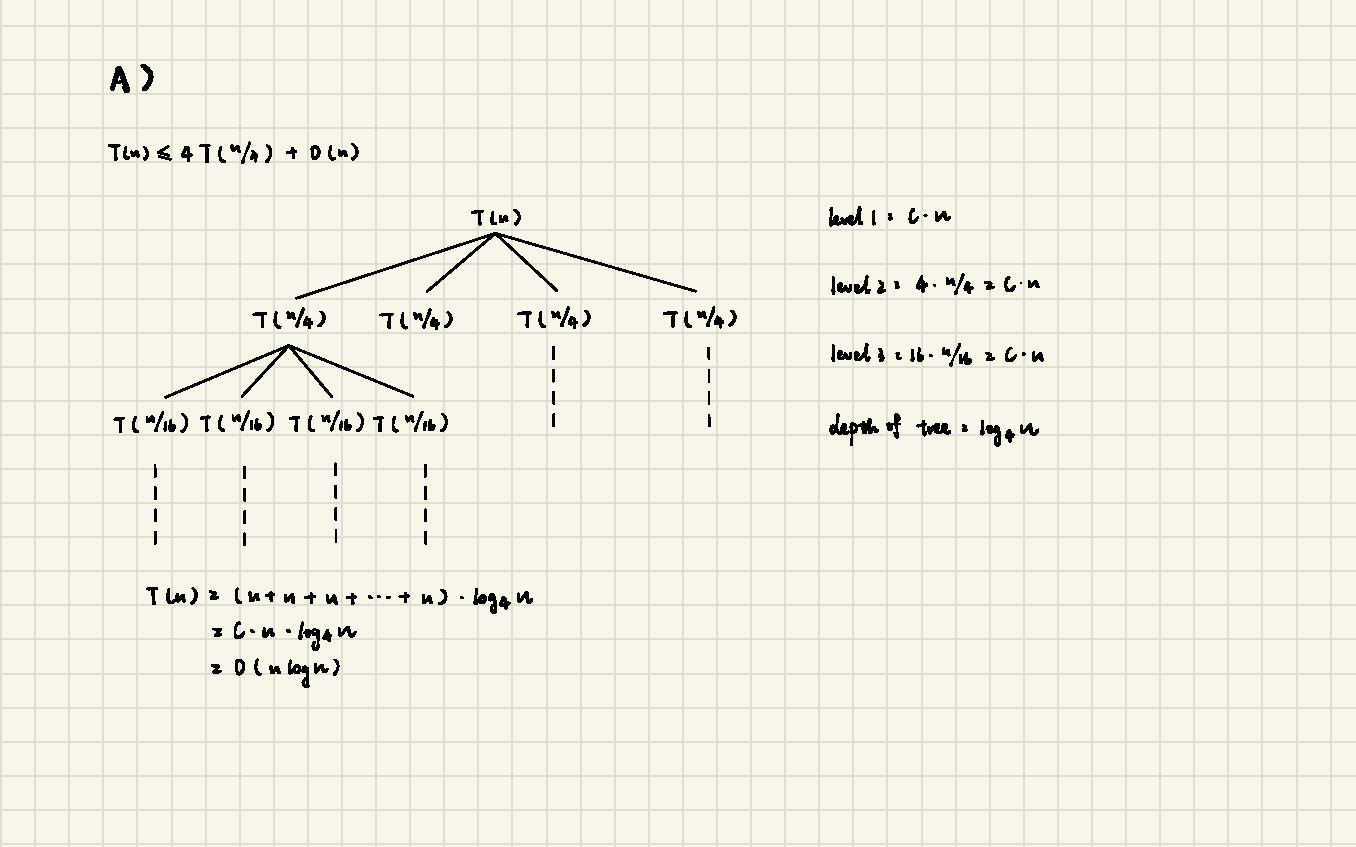
\includegraphics[width=0.8\textwidth]{treeA.pdf}}{No Figure Yet}
			\caption{Recursion tree for algorithm $A$.} 
		\end{figure}
		
\end{solution}

		\item Algorithm $B$ divides an instance of size $n$ into $2$ subproblems, one with size $n/4$ and one with size $n/5$, recursively solves each one, and then takes $O(n)$ time 
		to combine the solutions and output the answer. 
		
		    \begin{solution}
		    
		    	\emph{Runtime Analysis}
	
		\begin{figure}[h!]
			\centering
			\IfFileExists{treeB.pdf}{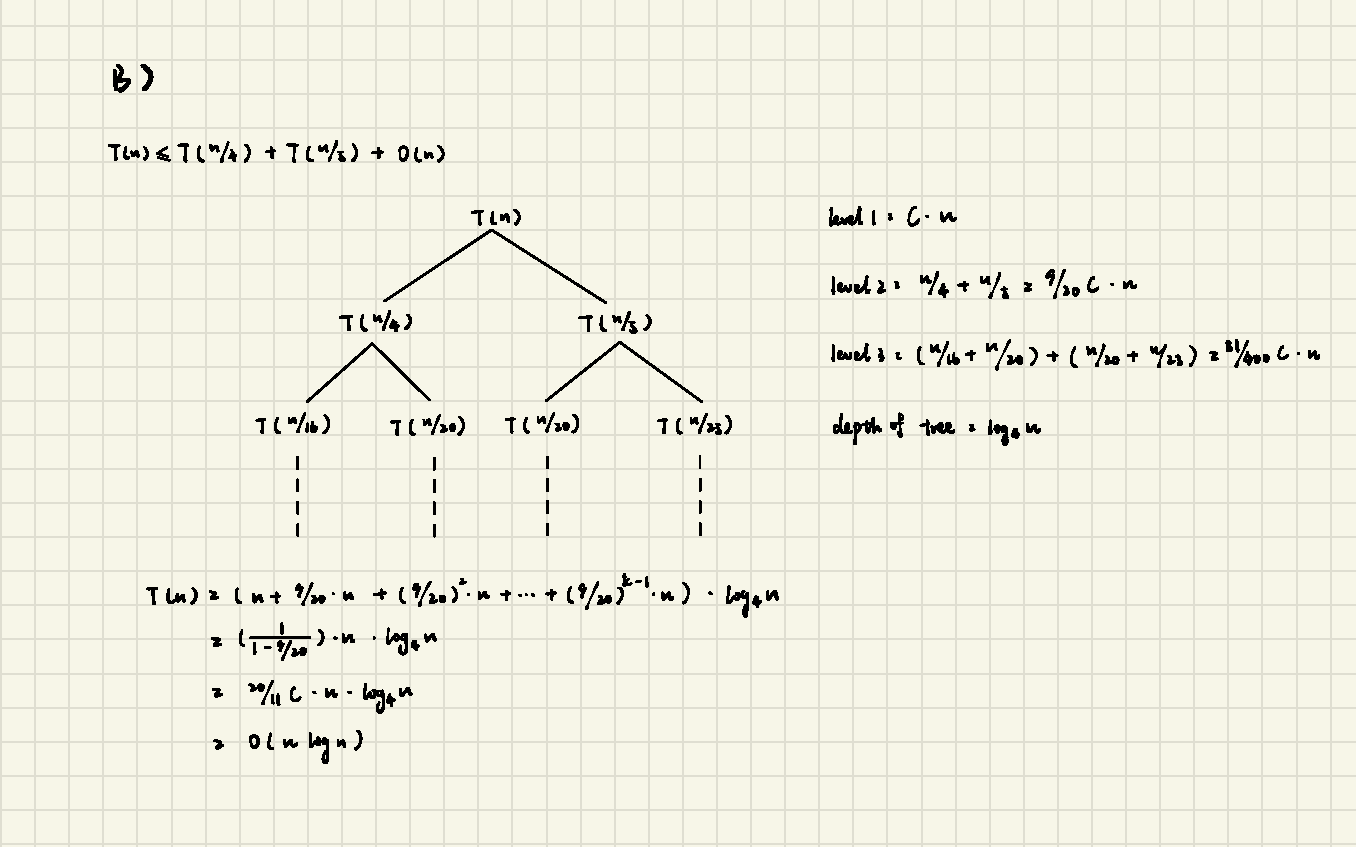
\includegraphics[width=0.5\textwidth]{treeB.pdf}}{No Figure Yet}
			\caption{Recursion tree for algorithm $B$.} 
		\end{figure}
		
\end{solution}

		\item Algorithm $C$ divides an instance of size $n$ into $4$ subproblems of size $n/3$ each, recursively solves each one, and then takes $O(n^2)$ time 
		to combine the solutions and output the answer. 
		
		    \begin{solution}
			
			\emph{Runtime Analysis}
	
		\begin{figure}[h!]
			\centering
			\IfFileExists{treeC.pdf}{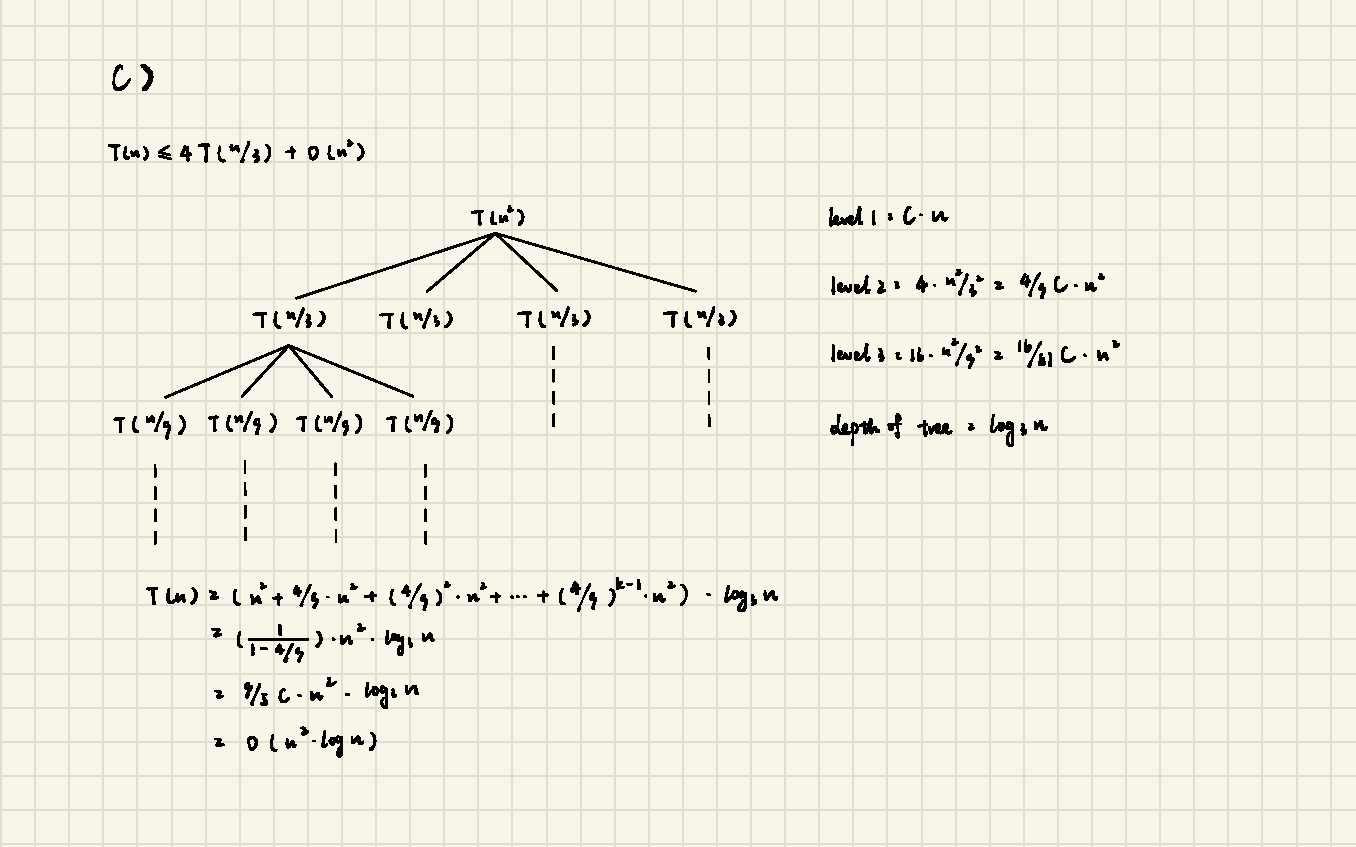
\includegraphics[width=0.5\textwidth]{treeC.pdf}}{No Figure Yet}
			\caption{Recursion tree for algorithm $C$.} 
		\end{figure}
\end{solution}

		\item Algorithm $D$ divides an instance of size $n$ in to $2$ subproblems of size $n-1$ each, recursively solves each one, and then takes $O(1)$ time to combine the solutions and output the answer. 
		
		    \begin{solution}

			\emph{Runtime Analysis}
	
		\begin{figure}[h!]
			\centering
			\IfFileExists{treeD.pdf}{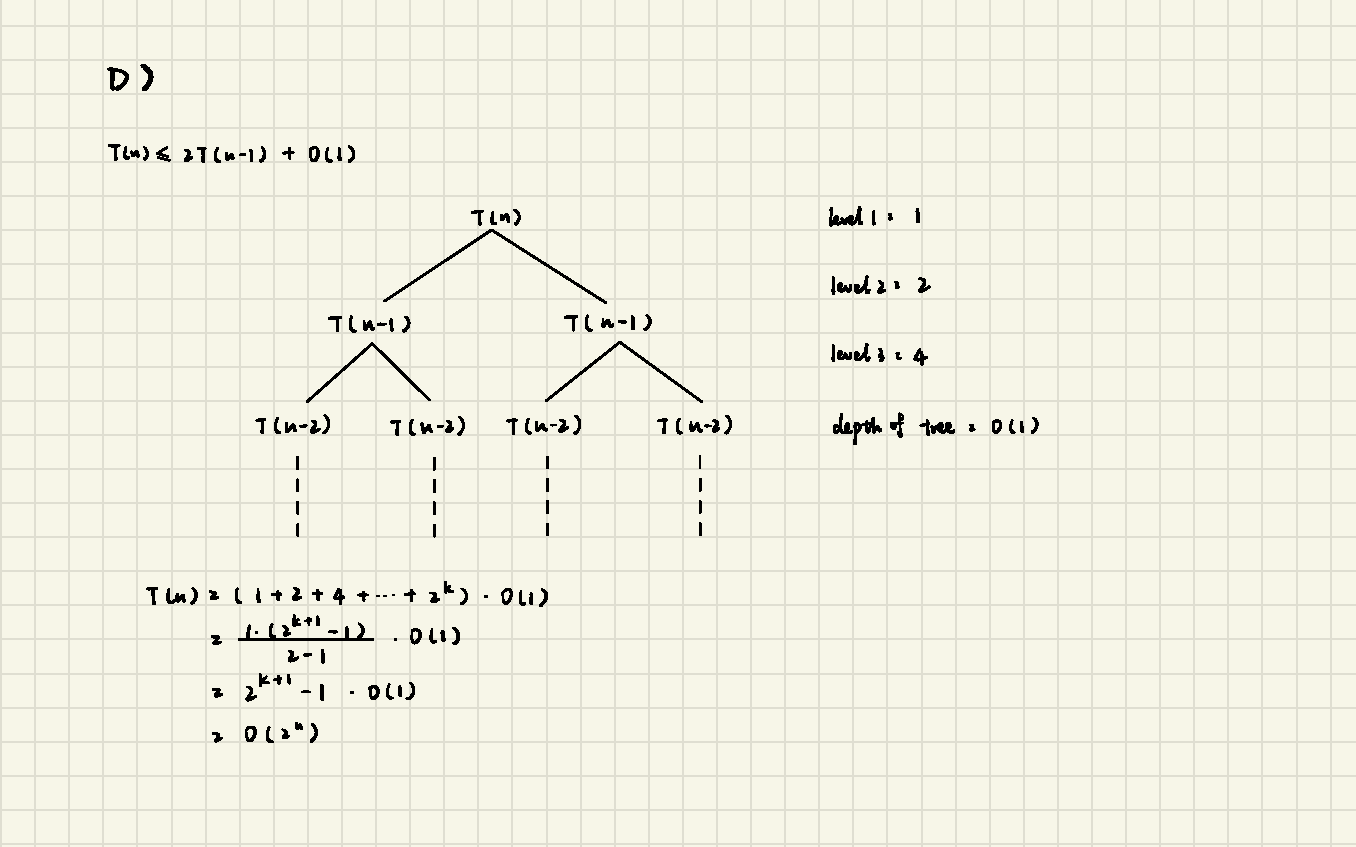
\includegraphics[width=0.5\textwidth]{treeD.pdf}}{No Figure Yet}
			\caption{Recursion tree for algorithm $D$.} 
		\end{figure}
\end{solution}

	\end{enumerate}
	
	For each algorithm, write a recurrence for its runtime and \emph{use the recursion tree method} of Lecture 3 to solve this recurrence and find the \emph{tightest asymptotic} upper bound on runtime of the algorithm. \grade{25} 
\end{problem}

\smallskip

\begin{problem}
	In this problem, we consider a non-standard sorting algorithm called the \emph{Silly Sort}. Given an array $A[1:n]$ of $n$ integers, the algorithm is as follows: 
	
	$\bullet$ \textbf{Silly-Sort}$(A[1:n])$:
	\begin{enumerate}
		\item If $n < 5$, run merge sort (or selection sort or insertion sort) on $A$.  
		\item Otherwise, run \textbf{Silly-Sort}$(A[1:3n/4])$, \textbf{Silly-Sort}$(A[n/4:n])$, and \textbf{Silly-Sort}$(A[1:3n/4])$ again. 
	\end{enumerate} 
	
	We now analyze this algorithm. 
	
	\begin{enumerate}
		\item [(a)] Prove the correctness of  \textbf{Silly-Sort}. \grade{10} 
		
	\begin{solution}
	
	\emph{Proof of Correctness} \\
		The proof of correctness is expressed by induction on n. For n = 2, namely the base case, the algorithm returns after the following sort. After the second recursive call, the n/4 largest elements of A will appear in sorted order in 		A[3n/4 + 1, ..., n]. Knowing that by the induction hypothesis the first call to Silly-Sort(A[1 : 3n/4]), the n/4 largest elements of A are in positions n/4 + 1, ..., n. Then, assuming that after the second recursive call, the n/4 largest 		elements of A are in their correct positions, and the third recursive call sorts correctly the elements 1 ... 3n/4 by induction hypothesis. Thus the array A of size n is sorted.
	
\end{solution}

		\item [(b)] Write a recurrence for  \textbf{Silly-Sort} and use the recursion tree method of Lecture 3 to solve this recurrence and find the \emph{tightest asymptotic} upper bound on the runtime of \textbf{Silly-Sort}. \grade{10}
		
	\begin{solution}
	
	\begin{figure}[h!]
			\centering
			\IfFileExists{sillySort.pdf}{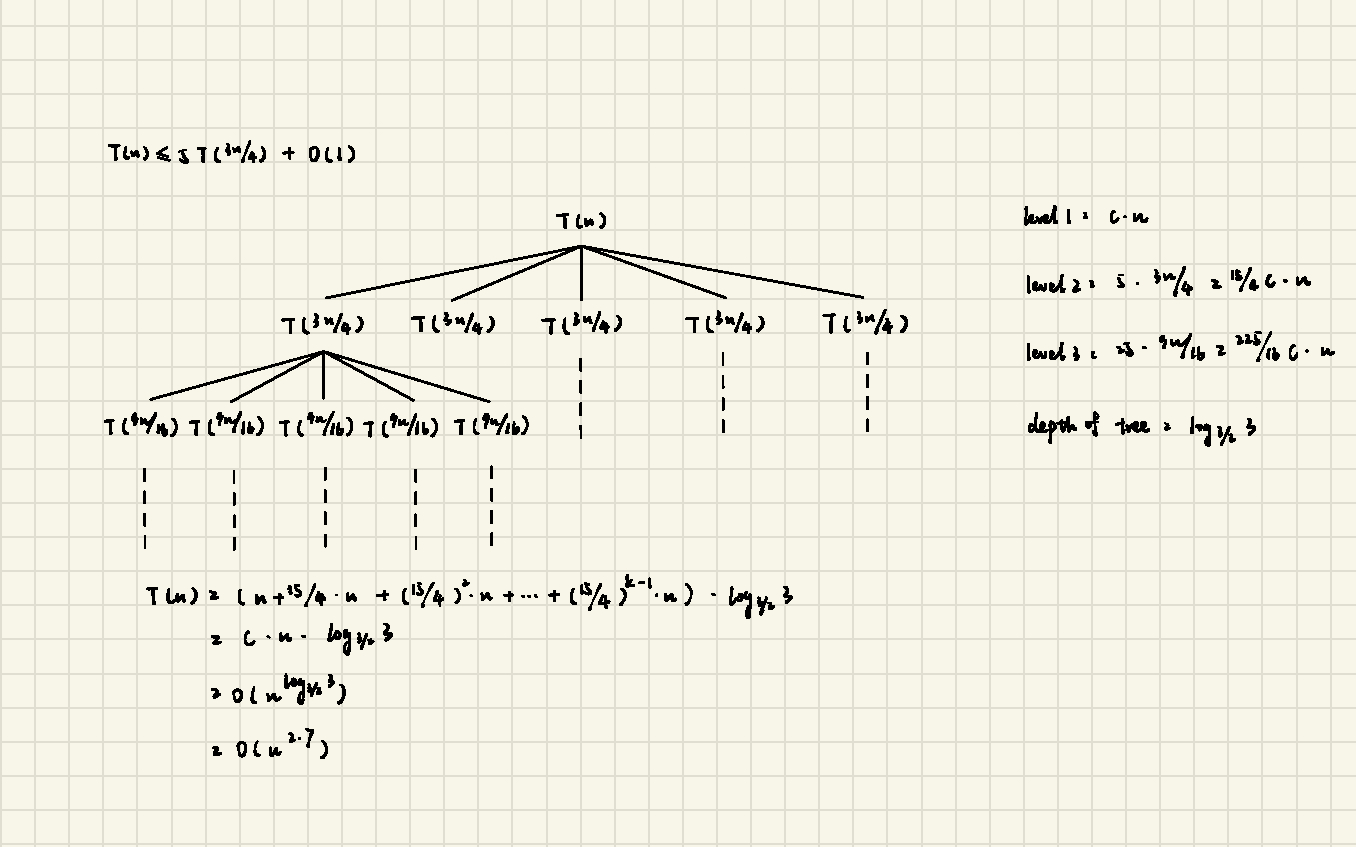
\includegraphics[width=0.5\textwidth]{sillySort.pdf}}{No Figure Yet}
			\caption{Recursion tree for Silly-Sort.} 
		\end{figure}
		
\end{solution}

		\item [(c)] Suppose we like to change the second line of the algorithm to 
		\[
		\text{\textbf{Silly-Sort}$(A[1:m])$, \textbf{Silly-Sort}$(A[n-m:n])$, and \textbf{Silly-Sort}$(A[1:m])$}
		\]
		 for some other value of $m$ instead (in the original algorithm, $m = 3n/4$). 
		
		What is the smallest number we could pick while still maintaining the correctness of the algorithm? What would be the runtime of the resulting algorithm? 
		For this part of the question, you can simply write a few lines for proof of 
		correctness and runtime analysis by pointing out how your proofs and calculations in parts (a) and (b) should be changed. \grade{5}
		
	 \begin{solution}
	 	The smallest number is m = 3n/4. 
		The proof of correctness is expressed by induction on n. For n = 2, namely the base case, the algorithm returns after the following sort. After the second recursive call, the n-m largest elements of A will appear in sorted order in 		A[m + 1, ..., n]. Knowing that by the induction hypothesis the first call to Silly-Sort(A[1 : m]), the n/4 largest elements of A are in positions n - m + 1, ..., n. Then, assuming that after the second recursive call, the m largest 			elements of A are in their correct positions, and the third recursive call sorts correctly the elements 1 ... m by induction hypothesis. Thus the array A of size n is sorted.

	
\end{solution}

	\end{enumerate}
\end{problem}

\smallskip

\begin{problem}
    You are given an array $A[1:n]$ which includes the scores of $n$ players in a game. They are ranked in the following way: 
    Rank of a player is an integer $r$ if there are exactly $r-1$ \emph{distinct} scores strictly smaller than the score of this player (irrespective of the number of players).
  
  \begin{enumerate}
  	\item[(a)] Design and analyze an algorithm that given the array $A$, can find the rank of all players in the array in $O(n\log{n})$ time. \grade{15}
    
    	\medskip
    
    \textbf{Example.} Suppose the input array is $A=[1,7,6,5,2,4,5,2]$ for 8 players; then the rank of  players is: 
    \begin{itemize}
        \item Player $A[1]$ has rank 1 (as $A[1]=1$ is the smallest number); 
        \item Player $A[2]$ has rank 6 (as $A[2]=7$ has $5$ distinct smaller numbers: $\set{1,6,5,4,2}$);
        \item Player $A[3]$ has rank 5 (as $A[3]=6$ has $4$ distinct smaller numbers: $\set{1,5,4,2}$);
        \item Player $A[4]$ has rank 4 (as $A[4]=5$ has $3$ distinct smaller numbers: $\set{1,4,2}$);
        \item Player $A[5]$ has rank 2 (as $A[5]=2$ has $1$ distinct smaller number: $\set{1}$);
        \item Player $A[6]$ has rank 3 (as $A[6]=4$ has $2$ distinct smaller numbers: $\set{1,2}$);
        \item Player $A[7]$ has rank 4 (as $A[7]=5$ has $3$ distinct smaller numbers: $\set{1,4,2}$);
        \item Player $A[8]$ has rank 2 (as $A[8]=2$ has $1$ distinct smaller number: $\set{1}$);
    \end{itemize}
    
    
    	 \begin{solution} .\\
	 1. Create another array B[n] of n size. \\
	 2. Copy array A to array B. \\
	 3. Sort elements in array B in ascending order using merge sort. \\
	 4. Traverse array B and put their rank in HashMap by taking a rank variable. \\
	 5. If the element isn't present in HashMap, update its rank in HaspMap and increment rank, otherwise do nothing. \\
	 6. Traverse array B and assign the rank of each element. \\
	 Time Complexity: $O(n\log{n})$ 
	
\end{solution}

    \item [(b)] Suppose you are additionally given an array $B[1:m]$ with the score of $m$ new players. Design and analyze an algorithm that given both arrays $A$ and $B$, can find the rank of each player $B$ inside the array $A$, i.e., 
    for each $B[i]$, determines what would be  the rank of $B[i]$ in the array consisting of all elements of $A$ plus $B[i]$. Your algorithm should run in $O((n+m) \cdot \log{n})$ time. \grade{10} 
      
      \medskip
  \textbf{Example.} Suppose the input array is $A=[1,7,6,5,2,4,5,2]$ as before and $B=[3,9,4]$; then the correct answer for each player in $B$ is: 
    \begin{itemize}
        \item Player $B[1]$ will have rank 3 (as $B[1]=3$ has $2$ distinct smaller numbers in $A$: $\set{1,2}$); 
        \item Player $B[2]$ will have rank 7 (as $B[2]=9$ has $6$ distinct smaller numbers in $A$: $\set{1,7,6,5,4,2}$);
        \item Player $B[3]$ will have rank 3 (as $B[3]=4$ has $2$ distinct smaller numbers in $A$: $\set{1,2}$);
    \end{itemize}
    
    
     	\begin{solution}.\\
		1. Sort the two arrays, and then use two pointers to traverse the two arrays. Predictably, the elements that join the array of answers must be incremental. \\ 
		2. In order to ensure the uniqueness of the joined elements, record the variable pre to represent the elements that last joined the array of answers. \\
		3. Initially, the two pointers point to the heads of the two arrays. Compare the numbers in the two arrays that the two pointers point to at a time, and if the two numbers are not equal, move the pointer to the smaller number one 		bit to the right. \\ 
		4. If the two numbers are equal and the number is not equal to pre, add the number to the answer and update the pre variable, and move both pointers one bit to the right. The traversal ends when at least one pointer is out of 		range of the array. \\
		5. Form a new array by looping through all elements. In each loop, the values of the p1 and p2 pointers in the two arrays are compared so that the current pointer always points to the next element of the smaller value element. 
		
\end{solution}

    
    \end{enumerate}
    
\end{problem}

%=====================================================
% LaTeX Tip: For problems that have a single part, write your solutions  in a solution environment, i.e., between a \begin{solution} and \end{solution} command, and define this command write AFTER the problem statement. 
%=====================================================	

\smallskip

\finishline

\begin{challenge}
	Let us revisit the community detection problem but with an interesting twist. Remember that we have a collection of $n$ people for some odd integer $n$ and we know that strictly more than half of them belong to a hidden community. 
	As before, when we introduce two people together, the members of the hidden community would say they know the other person if they also belong to the community, and otherwise they say they do not know the other person. 
	The twist is now as follows: the people that do not belong to the community \emph{may lie}, meaning that they may decide to say they know the other person even though in reality only people inside the hidden community know each other.
	
	Concretely, 
	suppose we introduce two people $A$ and $B$, then what they will say would be one of the following (first part of tuple is the answer of $A$ and second part is the answer of $B$): 
	\begin{itemize}
		\item if both belong: $(know~,~know)$;
		\item if $A$ belongs  and $B$ does not: $(does\ not\ know~,~know/does\ not\ know)$; 
		\item if $B$ belongs  and $A$ does not: $(know/does\ not\ know~,~does\ not\ know)$; 
		\item if neither belongs:  $(know/does\ not\ know~,~know/does\ not\ know)$; 
	\end{itemize}
	Design an algorithm that finds all members of the hidden community using $O(n)$ greetings. \grade{+10} 
	
	\begin{solution} .\\
		1. Pair the participants into groups of size two with one extra person with no group. Ask the pairs in each group to greet each other. If we found a group that know each other, let P be any arbitrary participant of this group. 			Otherwise let P be the extra person with no group. Repeat this process, let the re-combined P place in a separate group. (In this algorithm, P is supposed to denote a member of the hidden community) \\
		2. Ask P to greet everyone else. Mark whoever knows P plus P itself as the members of the all hidden community(including who lies). \\
		3. Then let number of the all hidden community greet each other again, find those who are the real one. 
	
	\end{solution} 
	
\end{challenge}

\begin{fun}
	We have an $n$-story building and a series of magical vases that work as follows: there is some unknown level $L$ in the building that if we throw these vases down from any of the levels $L,L+1,\ldots,n$, they will definitely break; however, 
	no matter how many times we throw the vases down from any level below $L$ nothing will happen them. Our goal in this question is to determine this level $L$ by throwing the vases from different levels of the building (!). 
	
	For each of the scenarios below, design an algorithm that uses asymptotically the smallest number of times we throw a vase (so the measure of efficiency for us is the number of vase throws). 
	\begin{enumerate}
	\item[(a)] When we have only one vase. Once we break the vase, there is nothing else we can do. \grade{+2} 
	
	
    	\begin{solution}
		For only one vase, we need to make sure the vase doesn't break until we determine the level L, meaning from level 1, level 2 and so on until level L. We need to throw the vase n times so that the time complexity = O(n).
\end{solution}


	\item[(b)] When we have  four vases. Once we break all four vases, there is nothing else we can do. \grade{+4} 
	

    	\begin{solution}
		For four vases, meaning we can break previous three but still be constant. Then we still need to test each floor until level L. Therefore the time complexity also = O(n).
\end{solution}


	\item[(c)] When we have an unlimited number of vases.  \grade{+4} 
	
	
    	\begin{solution}
		Now we have an unlimited number of vase, then we can use binary search to find the level L. So the building level to test decreases as $n/2 + n/4 + n/8 +....... (n/2)^k$. Solving this we get k to be log2(n), which means the time 		complexity = $O(\log n)$.
\end{solution}


	\end{enumerate}
\end{fun}
\end{document}





